\documentclass[11pt]{article}
\usepackage[margin=1in]{geometry}
\usepackage[utf8]{inputenc}
\usepackage[T1]{fontenc}
\usepackage{amsmath,amssymb,amsthm}
\usepackage{booktabs}
\usepackage{array}
\usepackage{enumitem}
\usepackage{graphicx}
\usepackage{xcolor}
\usepackage{tikz}
\usetikzlibrary{arrows.meta,positioning,fit,backgrounds}
\usepackage{algorithm}
\usepackage{algpseudocode}
\usepackage[colorlinks=true,linkcolor=blue!50!black,citecolor=blue!50!black,urlcolor=blue!50!black]{hyperref}
\usepackage{natbib}
\usepackage{microtype}
\emergencystretch=2.5em

\title{Evidence-Gated Prompt Optimization on a Synthetic Attractor Scaffold:\\
A Preprint of the \texttt{prompt-optimization} Toolkit}
% TODO(author): replace the placeholder author block with real names/affiliations.
\author{Author Name$^1$ \and Collaborator Name$^2$\\
\small $^1$Affiliation, $^2$Affiliation\\
\small \texttt{placeholder@example.org} % TODO(author): remove fake email
}
\date{\today}

\begin{document}
\maketitle

\begin{abstract}
How much of ``this prompt is better'' can a prompt-optimization pipeline actually
claim? \emph{prompt-optimization} is a reproducible Python scaffold for studying
prompt rate-distortion, behavioral attribution, and candidate selection. Its
pipeline scores discrete prompt candidates against a set of named behavioral
\emph{attractors} in a synthetic embedding model, attributes score differences to
prompt components, and selects candidates via an empirical distortion-rate
frontier, Pareto non-dominance, and \emph{mandatory hard gates} that no score may
override. This preprint documents that mechanism and architecture, gives one real
worked example (scoring the candidate files of an independent skill repository),
and -- the load-bearing part -- reports an explicit \emph{Evaluation Status}: the
toolkit validates \emph{implementation invariants only}. Its numbers are synthetic
attractor outputs, not measurements of any LLM. No real held-out model evaluation
exists yet; no pre-registered protocol exists yet; and the pipeline currently has
no architectural seam at which a real evaluator could \emph{dispose} of synthetic
proposals. We state these gaps as findings, in the spirit that characterizes this
line of research: behavioral performance must dominate embedding similarity, and
an absence of evidence is itself a reportable result.
\end{abstract}

Automatic prompt optimization has matured from token-level search
\citep{shin2020autoprompt} to an active subfield of generate-and-search
\citep{zhou2023ape,yang2023opro,fernando2023promptbreeder,guo2023evoprompt,pryzant2023protegi,khattab2023dspy,yuksekgonul2024textgrad},
with scoring functions that range from task accuracy to optimizer-LLM judgment.
A naive version of this loop has a quiet failure mode: the ranking step slowly
becomes ``how geometrically close is this candidate to a hand-defined target
embedding,'' and the whole enterprise quietly turns into a search for cosine
neighbors of one vector. The present project was motivated by the observation
that \emph{embedding similarity is not behavioral equivalence}
\citep{kornblith2019similarity}: a candidate can sit near a target direction and
be behaviorally inert, or sit far away and be behaviorally decisive. The design
stance of \texttt{prompt-optimization} is therefore that \emph{behavioral
performance must dominate embedding similarity}, and that any ordering signal
from embeddings must be re-grounded on real held-out evaluation before it
becomes a claim.

This preprint documents the toolkit as a \emph{research scaffold} for developing
and checking that ordering logic cheaply and reproducibly, before any expensive
real-model experiment is run. It makes three contributions, in the honest-scope
sense of \texttt{specimen}-style evaluation:

\begin{enumerate}[leftmargin=*]
  \item \textbf{A vocabulary and selection discipline} -- named behavioral
  attractors, basin probabilities, reliability and a deliberately-admitted-toy
  distortion proxy, plus empirical distortion-rate and Pareto selection with
  mandatory hard gates that no scalar score may override.
  \item \textbf{A shipped architecture and one real worked example} -- three
  subpackages (\texttt{metrics}, \texttt{attribution}, \texttt{context}), a
  stdlib-only CLI (\texttt{prompt-opt scan} / \texttt{plan}), and a genuine
  transcript of the tool being pointed at an independent skill repository.
  \item \textbf{An honest evaluation status} -- a classification of exactly what
  the shipped evidence licenses and what it does not, which doubles as a
  concrete fix list for turning this scaffold into a measurement device.
\end{enumerate}

The evaluation-status section is the point of this paper. The rest of the paper
is machinery; Section~\ref{sec:eval} is where the reader should look if they want
to know what this toolkit can and cannot yet claim.
Related work is organized by mechanism, not chronology. For each cluster we
state what the cited work \emph{establishes} and what it does \emph{not}, and we
flag the one correction to the project's own notes that surfaced during the
literature scan for this preprint.
\label{sec:rel}

\paragraph{Discrete prompt search (generate-and-search).} \citet{zhou2023ape}
introduced LLM-generated candidate prompts scored on task accuracy
\emph{(automatic prompt engineering)}; \citet{yang2023opro} framed the optimizer
itself as an LLM that proposes candidates from a scored history, and reported the
now-celebrated case where a short phrase (``take a deep breath'')
beat longer instructions. Later scale-limits work \citep{zhang2024reoprolim} shows
the optimizer's size and human-written meta-instructions strongly condition these
results --- a direct warning against letting a scaffold rank without stating its
evaluator. \citet{shin2020autoprompt} searched trigger tokens via gradients;
\citet{fernando2023promptbreeder} evolved prompts; \citet{guo2023evoprompt}
reused evolutionary operators; \citet{pryzant2023protegi} treated natural-language
critiques as ``gradients'' with beam search; \citet{khattab2023dspy} compiled
declarative LM programs; \citet{yuksekgonul2024textgrad} propagated textual
gradients through computation graphs; and \citet{latentprompt2025} searched a
continuous latent space and decoded candidates. What this cluster establishes:
discrete or latent prompt candidates can be searched and scored programmatically.
What it does \emph{not}: it does not establish \emph{which wording does the most
behavioral work per token}, and much of it scores on the same model that proposes,
leaving an evaluator-leakage risk that \citet{zhang2024reoprolim} makes concrete.

\paragraph{Compression and information-theoretic bounds.}
\citet{jiang2023llmlingua} estimate token importance to compress existing prompts
for inference cost; the strongest precedent for this project's distortion-rate
posture is \citet{nagle2024promptrates} (``Fundamental Limits of Prompt
Compression''), which derives the distortion-rate function for black-box prompt
compression as a linear program. That paper establishes a \emph{theoretical}
bound; this toolkit's \texttt{rate\_distortion\_frontier} is an \emph{empirical}
lower envelope, a strictly weaker object. \citet{tishby2000ib} provides the
Information Bottleneck complement (compress input while preserving relevant
information), and \citet{xie2021icl} supplies the theoretical intuition for why
specific wording narrows the effective output distribution. None of these
operations turns a synthetic simulator into evidence about a real model.

\paragraph{Model selection and uncertainty.}
\citet{akinwande2023pacbayes} show that a language-model prior plus a discrete
prompt yields PAC-Bayes generalization bounds usable for model selection --
relevant because selection-confidence needs a penalty for optimizing on the
selection set only. \citet{sabbatella2023bayesprompt} formulate discrete prompt
tuning as combinatorial Bayesian optimization over a continuous surrogate;
\citet{zhou2026bayespo} treat prompts as posterior samples with a language-model
prior (a 2026 result this project cites as \emph{research option}, not evidence).
\citet{angelopoulos2021conformal} give the split-conformal toolkit that the
project's \texttt{conformal\_radius} mirrors in code. These works establish
techniques for honest uncertainty; this project ships the \emph{machinery}, not
the calibrated real-world numbers.

\paragraph{Mechanism: why short words matter.}
\citet{kornblith2019similarity} show that representation-similarity measures such
as CKA do not track task-relevant behavioral similarity --- the paper this
project's ``similarity $\neq$ behavior'' stance leans on. Steering work
\citep{turner2023activation,li2023iti,zou2023repe,panickssery2023caa,meng2022rome}
operates by causal intervention on activations, \emph{not} prompt wording; this
project borrows only the measurement instinct (project a candidate's effect onto
a declared direction) and does not claim access to any production model's
activations. \citet{bartoszcze2025repe} provide the recent survey.

\paragraph{Evaluation robustness.}
\citet{wallace2024instructionhierarchy} show that the priority among
system/developer/user text is itself learned behavior; \citet{li2023promptinj}
show instruction-following degrades under conflicting embedded text (so
``off-target'' should include unauthorized or unsafe behavior, not only semantic
competitors); \citet{wu2023counterfactual} show that apparent reasoning can rely
on default-condition shortcuts, motivating held-out and counterfactual
evaluation rather than more examples from the same template.

\paragraph{Novelty claim (scoped and checkable).}
To our knowledge, no other shipped, reproducible scaffold combines (a) scoring
discrete prompt candidates against \emph{named behavioral attractors}, (b)
empirical distortion-rate \emph{plus} Pareto selection, (c) \emph{mandatory} hard
gates that veto candidates regardless of score, and (d) cooperative-game
attribution (Shapley, interaction, deletion, directional) under one
evidence-gated pipeline whose explicit rule is that embedding-based orderings
must be reconfirmed on real held-out evaluation before use. We assert this
narrowly for the specific combination as implemented in this repository -- not
for the research space generally, and not as any claim of intrinsic novelty for
any single component.

\begin{quote}
\textbf{Correction of record.} The project's own research notes
(\texttt{research-landscape.md} under \texttt{docs/current/}) cite APE as
arXiv:2210.03493. A
live arXiv API check for this preprint shows \texttt{2210.03493} is instead
\textit{Automatic Chain of Thought Prompting in Large Language Models}
\citep{zhuosheng2022autocot}; the correct APE identifier is arXiv:2211.01910
\citep{zhou2023ape}. The present paper cites the corrected ID; the note file
should be updated.
\end{quote}
The toolkit's vocabulary, quoted from its source where possible.

A prompt candidate is reduced to a \emph{state} in a synthetic embedding space.
Formally the scaffold defines:

\begin{itemize}[leftmargin=*]
  \item \textbf{Attractor} -- a named point $\mathbf{a}_k \in \mathbb{R}^D$
  representing a target behavioral disposition. The shipped set is
  \texttt{VERIFY\_PRIOR}, \texttt{CREATIVE}, \texttt{CAUTIOUS},
  \texttt{AUTHORITATIVE}, \texttt{TRUSTING}, with default dimension $D=32$.
  \item \textbf{Prompt} -- a dataclass of text, a token count, and an
  embedding bias; optional scalar \texttt{nonlinearity} modulates resonance.
  \item \textbf{Final state}. The candidate's latent landing point is
  \begin{equation}
    \mathbf{s} = \mathbf{b} + \mathbf{r}\,\bigl(1+\nu\log(1+\lVert\mathbf{r}\rVert)\bigr)
    \cdot \frac{1}{1+0.15\max(\text{tokens}-2,0)},
  \end{equation}
  where $\mathbf{b}$ is the baseline (here $\mathbf{0}$) and $\nu$ is the
  nonlinearity. Longer prompts are scaled down (an efficiency factor), which is
  the source of the density intuition.
  \item \textbf{Basin probability}. Cosine distance from $\mathbf{s}$ to each
  attractor center, then a max-subtracted softmax at temperature $T=10$:
  \begin{equation}
    p_k(\mathbf{s}) = \frac{\exp(-d_{\cos}(\mathbf{s},\mathbf{a}_k)/T)}
    {\sum_j \exp(-d_{\cos}(\mathbf{s},\mathbf{a}_j)/T)}.
  \end{equation}
  Together with the attractor center $\mathbf{a}_0$ (the \emph{target}), these
  yield the per-candidate metric vector, all from a single deterministic run:
  \texttt{target\_activation} $=p_0(\mathbf{s})$;
  \texttt{reliability} $=\mathrm{mean}_i\, p_0(\mathbf{s}+\varepsilon_i)$ for
  $\varepsilon_i\sim\mathcal{N}(0,0.15)$;
  \texttt{distortion} $=1-\texttt{reliability}$ (a deliberately-synthetic proxy,
  openly the toy case the project's own notes criticize);
  \texttt{off\_target} $=\max_{k\ne0}p_k(\mathbf{s})$;
  \texttt{variance\_penalty} $=\mathrm{std}_i\,p_0(\mathbf{s}+\varepsilon_i)$;
  \texttt{distribution\_shift} $=W_1(p_0(\text{noisy}),p_0(\text{noisy baseline}))$;
  \texttt{instruction\_density} $=\texttt{target\_activation}\cdot
  \texttt{reliability}/\max(\text{tokens},1)$;
  and the scalar \texttt{score} $=p_0\cdot\texttt{reliability}
  -w_{\text{off}}\,\texttt{off\_target}-w_{\text{var}}\,\texttt{variance\_penalty}$.
  Finally \texttt{synAlign} is the cosine of $\mathbf{s}$ onto the target center:
  it is the \emph{synthetic alignment signal}, an ordering heuristic for the
  machinery, and is labeled as such rather than as evidence.
\end{itemize}

The \emph{selection layer} refuses to reify any single scalar. It computes an
empirical distortion-rate curve (best distortion at or below each token budget),
the Pareto-non-dominated subset over
$\langle\texttt{target\_activation},\texttt{reliability}\rangle$ maximized and
$\langle\texttt{tokens},\texttt{off\_target},\texttt{variance\_penalty}\rangle$
minimized, and a next-experiment recommendation by uncertainty-weighted gain.
Two of its objects matter most for the paper's thesis:

\begin{itemize}[leftmargin=*]
  \item \textbf{Hard gates}. A mapping of metric keys to bounds. A candidate
  that violates any key is \emph{excluded unconditionally}; score cannot rescue
  it. This is the operational form of ``some constraints are
  $\le\delta_{\text{critical}}$, not tradeable objectives.''
  \item \textbf{Rate-distortion frontier}. An \emph{empirical} lower envelope
  over measured tokens, not Shannon's theoretical bound (the distinction is
  drawn explicitly against \citet{nagle2024promptrates} in
  Section~\ref{sec:rel}).
\end{itemize}

The \emph{attribution layer} provides component-level estimands over any supplied
value function $v$: cooperative-game Shapley values (exact permutation
enumeration when the coalitions are small, reproducible Monte-Carlo otherwise),
the second-order inclusion-exclusion interaction term
$v(\{i,j\})-v(\{i\})-v(\{j\})+v(\emptyset)$, a paired deletion estimand, and a
directional projection of an observed state change onto a declared target
direction. Critically, these estimators are \emph{value-function agnostic}: their
conclusions are only as valid as the $v$ supplied. Shapley over the synthetic
cosine score is not Shapley over held-out architectural behavior.

The \emph{context layer} is an order-aware variant of the same idea: a token
sequence is position-encoded, passed through multi-head scaled-dot-product
\emph{causal} self-attention, pooled to a normalized contextual vector, and
evaluated with the same attractor metrics; a KV-cache memoizes the per-token
projections so repeated evaluations are bit-identical to a from-scratch pass but
cheaper.
The shipped decomposition (from the package layout and modules, not re-derived):

\begin{itemize}[leftmargin=*]
  \item \texttt{prompt\_optimization.metrics} -- attractor simulation and
  evaluation (\texttt{basin.py}), uncertainty (\texttt{uncertainty.py}:
  bootstrap interval, conformal radius, 1-Wasserstein, robust summary), and
  selection (\texttt{optimize.py}: Pareto, rate-distortion, metamorphic
  consistency, hard gates, next-experiment).
  \item \texttt{prompt\_optimization.attribution} -- \texttt{shapley.py},
  \texttt{interaction.py}, \texttt{direction.py}.
  \item \texttt{prompt\_optimization.context} -- \texttt{attention.py},
  \texttt{sequence.py}, \texttt{cache.py} (order-aware token path).
  \item \texttt{prompt\_optimization.cli.py} -- the \texttt{prompt-opt} surface.
\end{itemize}

Figure~\ref{fig:pipeline} shows the intended control flow. The single most
important architectural fact -- and the paper's central evaluation finding -- is
the vertical boundary inside the figure: everything above it is \emph{built and
tested on synthetic data}; everything below it is \emph{described in prose only}.
The scaffold can \emph{propose}; nothing in the shipped code is a seam at which a
real held-out model evaluation could \emph{dispose}.

\begin{figure}[ht]
\centering
\resizebox{\textwidth}{!}{
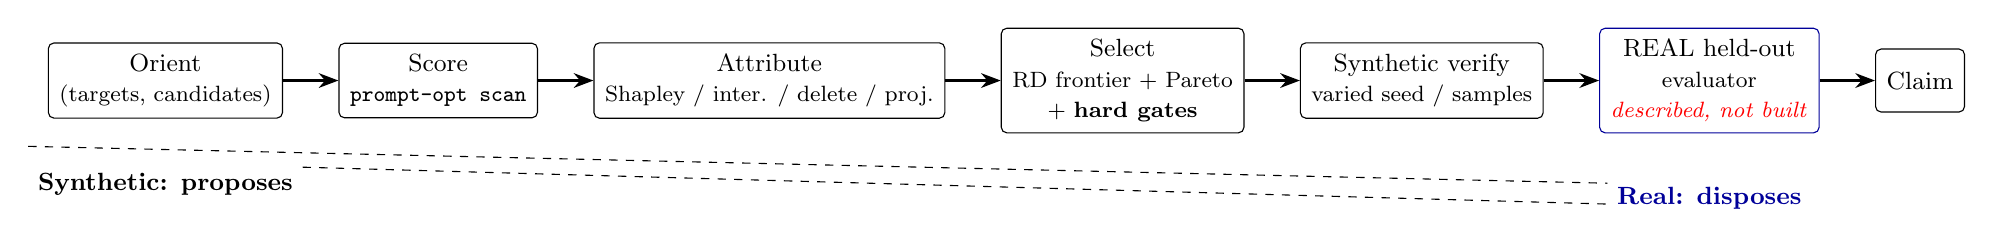
\begin{tikzpicture}[
  box/.style={draw, rounded corners=2pt, align=center, minimum height=8mm, inner sep=4pt},
  arr/.style={-{Stealth[length=2.5mm]}, thick},
  font=\small
]
\node[box] (orient) {Orient\\\footnotesize(targets, candidates)};
\node[box, right=2em of orient] (score) {Score\\\footnotesize\texttt{prompt-opt scan}};
\node[box, right=2em of score] (attr) {Attribute\\\footnotesize Shapley / inter. / delete / proj.};
\node[box, right=2em of attr] (sel) {Select\\\footnotesize RD frontier + Pareto\\\footnotesize + \textbf{hard gates}};
\node[box, right=2em of sel] (synv) {Synthetic verify\\\footnotesize varied seed / samples};
\draw[arr] (orient) -- (score);
\draw[arr] (score) -- (attr);
\draw[arr] (attr) -- (sel);
\draw[arr] (sel) -- (synv);

\node[box, draw=blue!60!black, right=2em of synv] (real) {REAL held-out\\\footnotesize evaluator\\\footnotesize \textcolor{red}{\emph{described, not built}}};
\node[box, right=2em of real] (claim) {Claim};
\draw[arr] (synv) -- (real);
\draw[arr] (real) -- (claim);

\node[below=1.6em of orient, font=\small\bfseries, align=center] (lbl1) {Synthetic: proposes};
\node[below=1.6em of real, font=\small\bfseries, text=blue!60!black, align=center] (lbl2) {Real: disposes};
\draw[dashed] ([yshift=0.6em]lbl1.north west) -- ([yshift=-0.2em]lbl2.north west);
\draw[dashed] ([yshift=0.6em]lbl1.east) -- ([yshift=-0.2em]lbl2.west);
\end{tikzpicture}}
\caption{The intended pipeline. The dashed vertical boundary separates the
synthetic scaffold (built and tested) from the real held-out evaluator (prose
only in the current codebase).}
\label{fig:pipeline}
\end{figure}

The pipeline underneath the CLI is deliberately deterministic and reproducible:
the same seed and sample count reproduce the same metric vector, and a
KV-cache guarantees bit-identical results between cached and from-scratch
context passes (verified by test). Nothing in the architecture pretends that the
synthetic attractor is a stand-in for a production model; the disclaimers in the
CLI output, the README, and the companion skill all say so in the same words:
\emph{synthetic scaffold: candidates only; real held-out evaluation disposes
before any claim}.
The public entry point is a stdlib-only command line (\texttt{prompt-opt
scan} / \texttt{prompt-opt plan}), installed as a console script from
\texttt{pyproject.toml}; \texttt{python -m prompt\_optimization ...} is
equivalent. The only third-party runtime dependency is NumPy.

\begin{table}[ht]
\centering
\small
\begin{tabular}{@{}l>{\raggedright\arraybackslash}p{3.4cm}>{\raggedright\arraybackslash}p{5.6cm}@{}}
\toprule
\textbf{Command} & \textbf{Flags} & \textbf{When to use} \\
\midrule
\verb|prompt-opt scan <paths...>| & \verb|--d-model| (must match attractor dim), \verb|--target|, \verb|--seed|, \verb|--samples|, \verb|--limit|, \verb|--json| &
per-candidate metric vector; the \texttt{synAlign} column is the synthetic alignment signal \\
\verb|prompt-opt plan <paths...>| & scan flags \textbf{plus} \verb|--gate KEY=BOUND| (repeatable), \verb|--gate-op max|min|, \verb|--json| &
hard-gate veto, then RD frontier + Pareto + next experiment \\
\midrule
\multicolumn{3}{@{}p{\textwidth}@{}}{\footnotesize Directories are walked
recursively; binaries, hidden files, and derived dirs (\texttt{.git},
\texttt{.venv}, \texttt{\_\_pycache\_\_}, \texttt{node\_modules}) are skipped.
``Tokens'' is a tokenizer-free estimate (word/punctuation count), explicitly not
a real tokenizer.}\\
\bottomrule
\end{tabular}
\caption{The \texttt{prompt-opt} surface.}
\label{tab:cli}
\end{table}

Two implementation details matter for the evaluation section. First, the
\emph{hard-gate} wiring was found buggy during preparation of this preprint (the
parser stored \texttt{--gate} under \texttt{args.gate}, but planning read
\texttt{args.gates}, so gates were silently never applied); the fix is in the
tree and covered by regression tests. Second, the human-readable scan table is
still \emph{sorted by \texttt{synAlign}} (cosine similarity), most-aligned first
-- an explicit remainder of the exact ranking role the project's own thesis says
should be demoted; the selection layer does not use it, but the display does.

The Python API re-exports the public surface at the top level
(\texttt{from prompt\_optimization import evaluate, pareto\_frontier,
shapley\_values, ContextCache, ...}), so all downstream code paths (metrics,
attribution, context) are importable without reaching into subpackages.
This section is a \emph{real transcript} -- the tool was actually run on
2026-08-28 against an independent target repository, the \texttt{specimen}
Claude Code skill (\texttt{Z:\textbackslash Specimen}), with the raw output files
preserved on disk under \texttt{output/specimen test 2/} in this project. It is
not a hand-traced walkthrough; the commands below are the ones that produced the
cited artifact files.

\textbf{Context.} \texttt{specimen} is an evidence-gated preprint skill: given a
project, it produces a paper that never claims more than the project's evidence
supports. Its repository contains seven candidate files (a \texttt{SKILL.md}, a
README, four \texttt{references/*.md} discipline documents, and one helper
script \texttt{scripts/arxiv\_lookup.py}). The question put to the scaffold was
the natural one: \emph{of these candidate formulations, which does the pipeline
favor under the default \texttt{VERIFY\_PRIOR} attractor, and is any selection
approximation to a behavioral preference?}

\begin{verbatim}
# 1. score every candidate file
prompt-opt scan --json Z:\Specimen
# 2. select over all candidates (permissive gate)
prompt-opt plan --gate distortion=0.8010 Z:\Specimen
# 3. select with a hard gate that only the cheapest point clears
prompt-opt plan --gate distortion=0.80065 Z:\Specimen
# 4. select with a strict hard gate every candidate fails
prompt-opt plan --gate distortion=0.7700 Z:\Specimen
\end{verbatim}

\textbf{Transcript highlights} (abridged; full artifact files
\texttt{scan.json}, \texttt{plan*.txt/json} are in \texttt{output/specimen test
2/}):

\begin{itemize}[leftmargin=*]
  \item The scan reported near-uniform metrics: the nontrivial spread was in
  \texttt{synAlign} (0.128 for README down to $-0.048$ for
  \texttt{latex-scaffold.md}); \texttt{target\_activation} sat in
  $[0.199,0.202]$, \texttt{reliability} in $[0.199,0.199]$, and therefore
  \texttt{distortion} in $[0.8006,0.8007]$ for every candidate. The frontier --
  best distortion at each token budget -- collapsed to a single repeated point:
  \texttt{README.md} at 303 tokens, distortion 0.8006, at \emph{every} budget.
  \item The Pareto-non-dominated set was \texttt{README.md} (303 tok, act 0.202),
  the \texttt{section-template.md} in \texttt{references/} (774 tok), and
  \texttt{scripts/arxiv\_lookup.py} (903 tok). The recommended next experiment
  was \texttt{README.md} (highest uncertainty-weighted gain, here tiny).
  \item With a hard gate at \texttt{distortion=0.80065}, exactly one candidate
  survives --- \texttt{README.md}; the other six are reported as \texttt{blocked}.
  \item With a hard gate at \texttt{distortion=0.77}, \emph{no} candidate
  survives, and the tool prints exactly the honest negative result:
  \texttt{"no candidate passes the hard gates ...; no supported improvement
  is claimed."}
\end{itemize}

\textbf{How to read this.} The transcript demonstrates that the machinery works
as specified: it scans, it gates (hard), it builds a frontier, and --- the most
specimen-native behavior --- it is willing to \emph{lose} loudly rather than
force a winner. It equally demonstrates that, at this attractor layout and
dimension, the scaffold has almost no discrimination: a narrow rounding margin
decides which single candidate survives a meaningful gate, and the frontier is a
constant. That is a property of the \emph{synthetic scaffold}, not of the
\texttt{specimen} skill; under no reading are these numbers evidence that
\texttt{README.md} ``causes more verify-prior behavior.'' They are evidence that
the ordering/selection logic runs and respects its gates.
\label{sec:eval}

This section is written to the discipline of \emph{evidence-status}: it reports
what evidence exists, classified by what each piece \emph{licenses}, and it ends
with an explicit claim boundary. The reminder that opens it is the discipline's
reflexive principle applied to this paper: a preprint arguing that engineering
claims should be evidence-gated must itself be evidence-gated, or it is doing
exactly the thing it warns about. The sections above are machinery; the claims
below are what the reader may actually rely on.

\subsection{Step 0: first-party evidence produced for this preprint}

\begin{enumerate}[leftmargin=*]
  \item \textbf{Test suite, re-run} on 2026-08-28: \texttt{46 passed}
  (5 test modules). Exercised through the package's public interface, including
  determinism, normalization, metric bounds, zero-token handling, Pareto /
  rate-distortion invariants, hard-gate wiring, JSON emission purity, attention
  masking, and KV-cache bit-identity.
  \item \textbf{CLI usage transcripts} on 2026-08-28, preserved on disk
  (\texttt{output/specimen test 2/}): \texttt{scan} and \texttt{plan} runs with
  three gate regimes against the \texttt{specimen} skill repository (Section 6).
\end{enumerate}

\subsection{Step 1--2: evidence inventory and classification}

\begin{table}[ht]
\centering
\small
\begin{tabular}{@{}p{4.0cm}>{\raggedright\arraybackslash}p{3.2cm}>{\raggedright\arraybackslash}p{5.4cm}@{}}
\toprule
\textbf{Evidence} & \textbf{Status} & \textbf{What it licenses} \\
\midrule
Pre-registered protocol & none & --- \\
Dated results log / case study & none & --- \\
Executed behavior (test suite) & 46/46 pass, 2026-08-28 & the exercised invariants behaved this way; NOT general correctness \\
Executed behavior (CLI runs) & gate regimes behaved as specified, dated & ordering/gating logic runs and respects hard gates; NOT ``these prompts are better'' \\
Static structure (lint/type checks) & none declared & --- \\
Empirical measurement (real model) & none & --- \\
Attribution outputs & subroutines covered by 3 tests & the estimators compute their defined quantities; NOT causal findings about prompts \\
Model/LLM judgment & none collected & --- \\
Human decision & one external adversarial skill review (2026) + this preprint & an accountable person accepted the design stance; NOT that the stance is validated \\
\bottomrule
\end{tabular}
\caption{Evidence classification for \texttt{prompt-optimization} (2026-08-28).}
\label{tab:evidence}
\end{table}

A single row must not be written up as if it answered a question from a
different row. The test suite licenses \emph{``the exercised cases behaved this
way''} and nothing about whether the toolkit improves any real prompt. The CLI
transcripts license \emph{``the selection logic ran and respected its gates''}
and nothing about the \texttt{specimen} repository being optimized.

\subsection{Failures of record (reported, not papered over)}

\begin{itemize}[leftmargin=*]
  \item \textbf{Stale/mislabeled citation in the project's own notes.}
  \texttt{research-landscape.md} (under \texttt{docs/current/}) cites APE as
  arXiv:2210.03493; the
  live arXiv API identifies that ID as \emph{Automatic Chain of Thought
  Prompting}, and APE is 2211.01910 (Section 2).
  \item \textbf{Hard-gate wiring bug (fixed).} Planning read
  \texttt{args.gates} while parsing stored \texttt{args.gate}, so
  \texttt{plan --gate ...} silently did nothing. Found while preparing this
  preprint's worked example; fixed; two regression tests added.
  \item \textbf{JSON pollution (fixed).} The strict-gate JSON path printed a
  human line to stdout before the JSON document, corrupting machine output. Fixed
  and covered by the same regression tests.
  \item \textbf{Missing top-level export (fixed).} \texttt{apply\_hard\_gates}
  was importable from the \texttt{metrics} subpackage but not re-exported at the
  package root, breaking a test import.
\end{itemize}

These are reported \emph{because} a fix list is the deliverable of an honest
evaluation status section: the first item is a documentation defect still in the
tree; the other three are defects already corrected, kept as findings of record.

\subsection{Claim boundary}

\emph{The mechanisms above are individually grounded in a passing test suite and
in the project's own design notes. They do not establish that
\texttt{prompt-optimization} improves any outcome on any real language model, nor
that any candidate ranking it produces reflects behavioral equivalence under
held-out evaluation. That is an open, and not yet even designed, empirical
question --- and, as the pipeline architecture itself insists, claimed performance
requires a real held-out evaluator to dispose of synthetic proposals before the
claim exists.}

The absence this section documents is not a defect in the writeup; per the
skill's own philosophy it is the finding: the toolkit's value today is as a
deterministic harness for developing ordering and selection logic, and its next
milestone is a real evaluation seam, not more math.
\paragraph{The synthetic evaluator is a stagehand, not a measure.}
\texttt{basin\_probabilities} is a softmax over cosine distances from
content-derived embeddings to five hand-placed centers at $D=32$;
\texttt{distortion = 1 - reliability} is, by the project's own admission in
\texttt{docs/current/research-landscape.md}, a toy proxy until a
task-specific behavioral distortion is defined. No threshold in this paper
(including the \texttt{0.80065} gate in the worked example) is calibrated
against anything.

\paragraph{Discrimination collapse.} In the worked example every candidate's
\texttt{distortion} landed in $[0.8006,0.8007]$: the metric space is
effectively flat at the tested dimension/layout, the rate-distortion frontier is
a constant, and gate membership is decided by rounding. A scaffold that cannot
separate candidates cannot be trusted to rank candidates; this is a concrete
threat to the validity of \emph{any} ordering the current scaffold emits and
should be on the front page of any future real test.

\paragraph{Embedding similarity still holds an ordering role.}
The human-readable scan table is sorted by \texttt{synAlign} (cosine), the
exact ``most-aligned first'' posture the project's thesis argues against
(Section 5). The selection layer ignores it, but a naive reader of the scaffold
output can still be misled into reading the display's first row as the
``answer.''

\paragraph{No real-evaluator seam.}
There is no interface, protocol, or CLI flag through which a real held-out
model evaluation can be supplied; the ``real held-out evaluation disposes''
language exists only in README/CLI prose (Section 4, Figure~\ref{fig:pipeline}).
A skill (the companion \texttt{specimen-prompt-eval}) that tells an agent to run
step ``verify (real)'' currently has no concrete command to give.

\paragraph{Attribution is value-function-agnostic but under-plumbed.}
The estimators are correct for their definitions, but nothing ships an example
value function, and no CLI path exists; an agent cannot currently exercise
attribution without reading package source.

\paragraph{Other scope boundaries.}
Tokenizer-free token estimates; a Windows-tested, single-numpy-dependency
environment; no lint/type-check step committed; no pre-registration (risk of
post-hoc fitting to attractor placement); the worked example was run before the
gate bug was fixed, so its permissive-gate numbers are the fixed behavior
re-verified on 2026-08-28.
The evaluation gap in Section 7 maps to concrete work, ordered by the leverage
it would buy. Each item is a \emph{proposal}, not a built feature.

\paragraph{1. Build the real-evaluator seam (highest leverage).}
Add a minimal \texttt{Evaluator} protocol and a \texttt{prompt-opt plan
--backend <adapter>} hook so a real held-out model (or a human-judged rubric)
can be plugged into the pipeline's \emph{dispose} position. Then make the
pipeline refuse to emit a ``selection'' as a claim unless a real run is present.
This is the review's centerpiece: \emph{synthetic optimizer proposes; real
held-out evaluator disposes}. Without the seam, the pipeline's own central rule
is aspirational.

\paragraph{2. Expose attribution through the CLI.}
A \texttt{prompt-opt attribute} subcommand with a shipped example value function
(and its limitations) would make the attribution layer executable by the same
agents who run \texttt{scan}/\texttt{plan}, closing the gap that currently
forces reading source.

\paragraph{3. De-rank the display.}
Stop sorting the scan table by \texttt{synAlign}; sort by a behavioral or
score-based ordering, or leave rows in corpus order. This closes the gap between
the thesis and the last place embedding similarity still outranks behavior.

\paragraph{4. Pre-register before measuring.}
Draft and date a protocol (task population, comparator, outcome measures,
stopping rule, a commitment to report null and adverse results) \emph{before}
collecting real-model data -- per the evidence-status discipline, to convert
``we have no evidence yet'' into a checkable plan rather than a permanent hedge.

\paragraph{5. Run two model families on held-out tasks.}
Evaluate the surviving candidates on unseen tasks across at least two model
families, report bootstrap intervals around each Pareto front point, and keep
optimizer and evaluator disjoint (the OPRO scale-limits warning,
\citet{zhang2024reoprolim}). Only then fit any activation probe.

\paragraph{6. Housekeeping.}
Fix the APE identifier in \texttt{docs/current/research-landscape.md}; add a
committed lint/type-check step; consider a task-specific behavioral distortion
measure to replace \texttt{1 - reliability}.

None of items 1--3 requires new mathematics; all three are architectural, which
is exactly where this project's next step lies.
\texttt{prompt-optimization} is a deterministic, reproducible scaffold for
developing the ordering and selection logic of evidence-gated prompt
optimization: name behavioral attractors, score candidates, attribute
differences, select on a distortion-rate and Pareto frontier with mandatory hard
gates that no score overrides, and \emph{never} promote a synthetic ordering to a
performance claim. Its evaluation status is honest rather than flattering: the
shipped evidence is a passing invariant suite and real CLI transcripts on a
synthetic scaffold; there is no real held-out model measurement, no
pre-registered protocol, and no seam yet at which a real evaluator could dispose
of synthetic proposals. Those are findings, and the concrete fix list that
closes them is the next contribution this line of work should make.

\bibliographystyle{plainnat}
\bibliography{refs}

\end{document}